% PROJECT INSTRUCTIONS PDF:
%       https://sakailogin.nd.edu/access/content/group/FA20-CSE-40647-CX-01/Logistics/project_instruction-fa

% ==============
% FROM SYLLABUS:
% ==============

% Course Project Policies:
% Grading distribution
%       Proposal Paper (10%), Milestone Paper (30%), Final Presentation (20%)
%       Final Paper (30%), Code/Data (10%), Discussion bonus (+3%)
% Teaming: each graduate team should have 2 to 3 students.

% • Proposal
%   o Paper (PDF): title, problem definition, potential solutions, data sources,
%       proposed evaluation methods, project plan/timeline
% • Milestone
%   o Paper (PDF): introduction, related work, problem definition, one or more
%       method that has been used, some other potential solutions, data and
%       experiment settings, evaluation methods, preliminary results and
%       experimental analysis, timeline.
%   o Presentation (PPTX) for selective projects: in class
% • Final
%   o Paper (PDF): introduction, related work, problem definition,
%       solutions and methods that have been used, data and
%       experiment settings, evaluation methods, experimental
%       results and analysis (tables and figures), discussion and
%       future work, conclusions
%   o Presentation (PPTX): in class.
% • Data and code package (ZIP):
% 
% • The papers (PDF) should be formatted according to the new Standard ACM Conference
% Proceedings Template: https://www.acm.org/publications/proceedings-template
% 
% • There will be -33% penalty if the paper is not formatted correctly.
% 
% • Deadlines
%       Every project required item is due at midnight (11:55pm) with
%       some grace period. There will be -33% penalty for each 24h past the deadline.

% ========================= GRADING =========================

% Both milestone paper and final paper will be graded using the project paper rubric.
% Note that the ACM template adoption is a pre-assumed metric for all the papers.

% The project presentation will be graded as follows:
%   Introduction: 15% Provide context. What questions are being addressed?
%   Solution/Method: 30%
%       What did you do? Why did you choose this method? What tools and techniques
%       did you use?
%   Data and Experiments: 10% What data did you use? Are your experimental methods reliable?
%       Evaluation and Results: 30% What evaluation did you do? Do your conclusions match your results?
%   Presentation Quality: 15% Clarity of speaking (5%), organization (5%), and visuals (5%).

% The project paper will be graded as follows:
%   Introduction: 15%
%       Provide context and motivation. What questions are being addressed? Why are
%       these questions interesting or important?
%   Related Work: 10%
%       What other methods have addressed these or similar questions? How do these
%       methods differ from your method?
%   Solution/Method: 25%
%       What did you do? What tools and techniques did you use? Was any innovation
%       attempted?
%   Data and Experiments: 10%
%       What data did you use? Are your experimental methods reliable? What
%       preprocessing was done the data?
%   Evaluation and Results: 25%
%       Did you properly evaluate your experiments? Did you test for statistical
%       significance? Do your conclusions match your results?
%   Writing Quality: 15% Clarity of writing (5%), organization (5%), and grammar (5%).

% \documentclass[acmsmall,authordraft]{acmart}
\documentclass[sigconf]{acmart}

    \newcommand{\guide}[0]{{\highlight{~\textsc{Guide}~}}}
\newcommand{\source}[1]{{\footnotesize \highlight{~\textsc{Source:}~#1~}}}

    \usepackage{lipsum}

% Easy Review:
% http://mirrors.ibiblio.org/CTAN/macros/latex/contrib/easyreview/doc/easyReview.pdf
\let\comment\undefined
\usepackage{easyReview}

% NOTE that a single column version is required for submission and peer review. This can be done by changing the \doucmentclass[...]{acmart} in this template to 
% \documentclass[manuscript,screen]{acmart}

%%
%% \BibTeX command to typeset BibTeX logo in the docs
\AtBeginDocument{%
  \providecommand\BibTeX{{%
    \normalfont B\kern-0.5em{\scshape i\kern-0.25em b}\kern-0.8em\TeX}}}

%% Rights management information.  This information is sent to you
%% when you complete the rights form.  These commands have SAMPLE
%% values in them; it is your responsibility as an author to replace
%% the commands and values with those provided to you when you
%% complete the rights form.
% \setcopyright{acmcopyright}
% \copyrightyear{2018}
% \acmYear{2018}
% \acmDOI{10.1145/1122445.1122456}

%% These commands are for a PROCEEDINGS abstract or paper.
% \acmConference[Woodstock '18]{Woodstock '18: ACM Symposium on Neural
%   Gaze Detection}{June 03--05, 2018}{Woodstock, NY}
% \acmBooktitle{Woodstock '18: ACM Symposium on Neural Gaze Detection,
%   June 03--05, 2018, Woodstock, NY}
% \acmPrice{15.00}
% \acmISBN{978-1-4503-XXXX-X/18/06}

%%
%% Submission ID.
%% Use this when submitting an article to a sponsored event. You'll
%% receive a unique submission ID from the organizers
%% of the event, and this ID should be used as the parameter to this command.
%%\acmSubmissionID{123-A56-BU3}

%%
%% The majority of ACM publications use numbered citations and
%% references.  The command \citestyle{authoryear} switches to the
%% "author year" style.
%%
%% If you are preparing content for an event
%% sponsored by ACM SIGGRAPH, you must use the "author year" style of
%% citations and references.
%% Uncommenting
%% the next command will enable that style.
%%\citestyle{acmauthoryear}

    
    \begin{document}
    
        %%
%% The "title" command has an optional parameter,
%% allowing the author to define a "short title" to be used in page headers.
\title[Data Science Project]{Our Awesome Data Science Project}

%% The "author" command and its associated commands are used to define
%% the authors and their affiliations.
%% Of note is the shared affiliation of the first two authors, and the
%% "authornote" and "authornotemark" commands
%% used to denote shared contribution to the research.

\author{Lucas Parzianello}
\affiliation{%
  \institution{University of Notre Dame}
  % \streetaddress{8600 Datapoint Drive}
  \city{Notre Dame}
  \state{Indiana}
  \postcode{46556}}
\email{lbarbosa@nd.edu}

\author{Sophia Abraham}
\affiliation{%
  \institution{University of Notre Dame}
  \city{Notre Dame}
  \state{Indiana}
  \postcode{46556}}
\email{?@nd.edu}

\author{Eric Tsai}
\affiliation{%
  \institution{University of Notre Dame}
  \city{Notre Dame}
  \state{Indiana}
  \postcode{46556}}
\email{?@nd.edu}

%%
%% By default, the full list of authors will be used in the page
%% headers. Often, this list is too long, and will overlap
%% other information printed in the page headers. This command allows
%% the author to define a more concise list
%% of authors' names for this purpose.
\renewcommand{\shortauthors}{Parzianello, Abraham, and Tsai.}

%%
%% The abstract is a short summary of the work to be presented in the
%% article.
\begin{abstract}
  \lipsum[1]
\end{abstract}

%% Generate the section below at http://dl.acm.org/ccs.cfm.
\begin{CCSXML}
<ccs2012>
<concept>
<concept_id>10010147.10010257</concept_id>
<concept_desc>Computing methodologies~Machine learning</concept_desc>
<concept_significance>300</concept_significance>
</concept>
<concept>
<concept_id>10010147.10010178.10010224</concept_id>
<concept_desc>Computing methodologies~Computer vision</concept_desc>
<concept_significance>500</concept_significance>
</concept>
<concept>
<concept_id>10010147.10010178.10010205</concept_id>
<concept_desc>Computing methodologies~Search methodologies</concept_desc>
<concept_significance>300</concept_significance>
</concept>
</ccs2012>
\end{CCSXML}

\ccsdesc[300]{Computing methodologies~Machine learning}
\ccsdesc[500]{Computing methodologies~Computer vision}
\ccsdesc[300]{Computing methodologies~Search methodologies}

%%
%% Keywords. The author(s) should pick words that accurately describe
%% the work being presented. Separate the keywords with commas.
\keywords{datasets, neural networks, gaze detection, text tagging}

%% A "teaser" image appears between the author and affiliation
%% information and the body of the document, and typically spans the
%% page.
% \begin{teaserfigure}
%   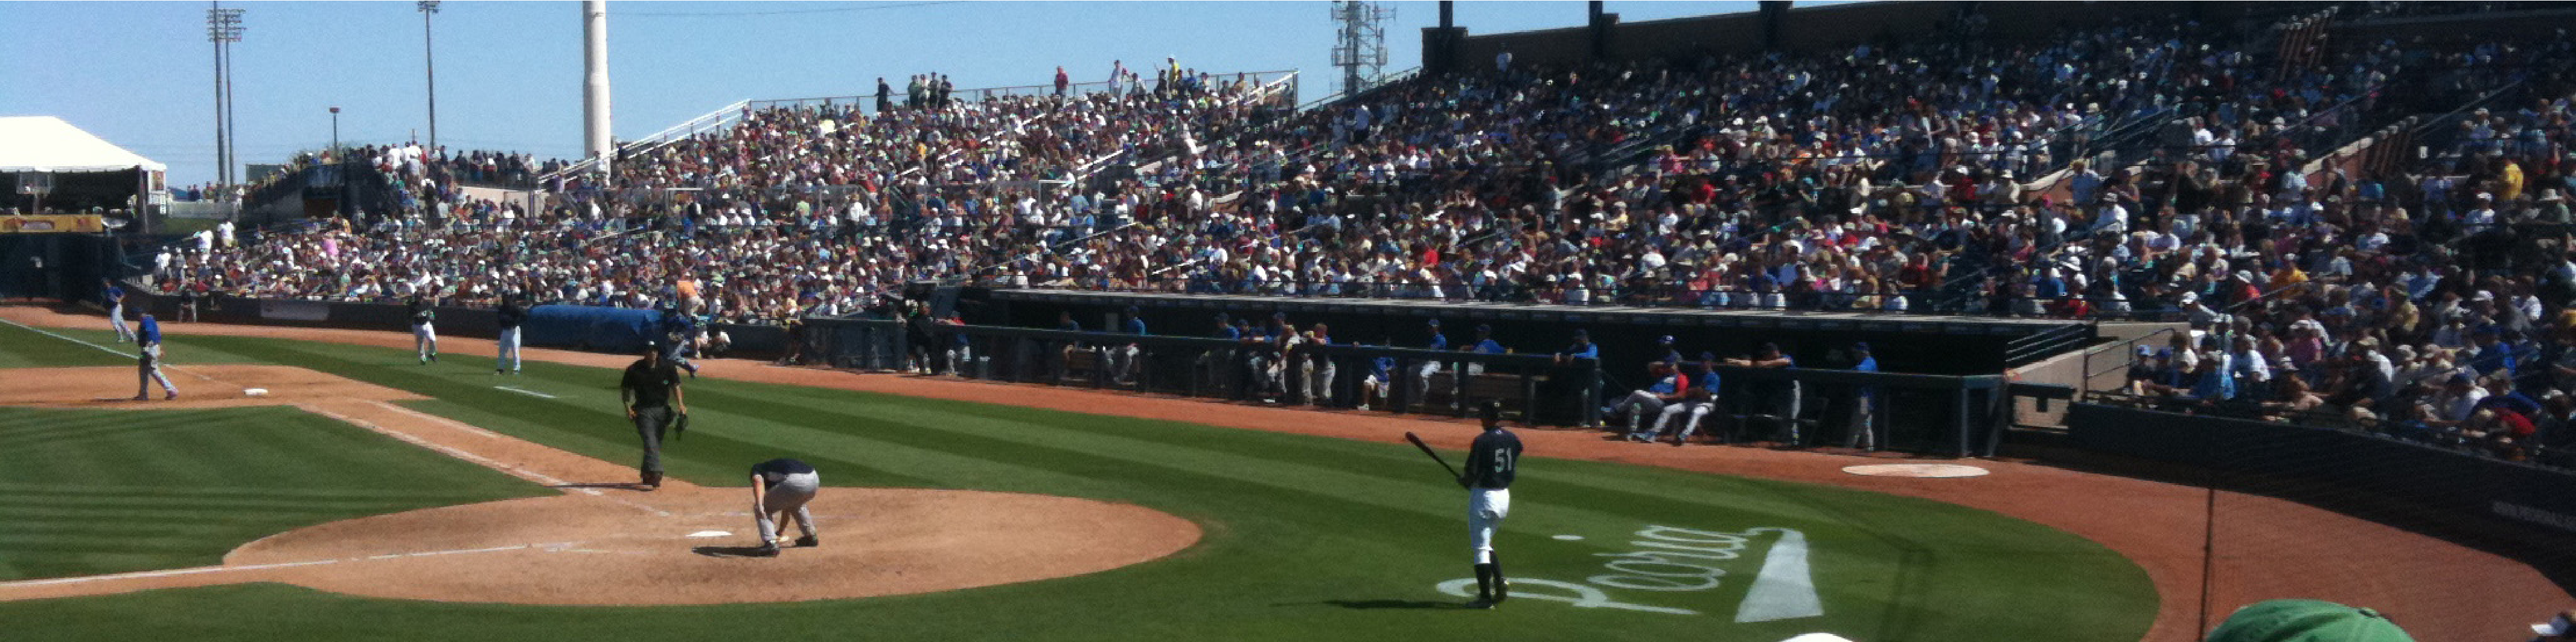
\includegraphics[width=\textwidth]{images/sampleteaser}
%   \caption{Seattle Mariners at Spring Training, 2010.}
%   \Description{Enjoying the baseball game from the third-base
%   seats. Ichiro Suzuki preparing to bat.}
%   \label{fig:teaser}
% \end{teaserfigure}

%%
%% This command processes the author and affiliation and title
%% information and builds the first part of the formatted document.
\maketitle

    
        % PROPOSAL:
        \section{Introduction}

\lipsum[2-6]

        \section{Related Work}

\subsection{Common classification methods}

In \citet{Bahuleyan2018}, they explore the application of machine learning (ML) algorithms to identify and classify the genre of a given audio file. The conventional ML models that are often seen are Gradient Boosting, Random Forests (RF), Logistic Regression (LR), and Support Vector Machines (SVM). This paper mainly compares the performance of two different classes of methods:
\begin{itemize}
    \item The first is to make prediction of the genre solely based on its spectrogram as input.
    \item The second approach is to make prediction of the genre based on features from frequency and time domain.
\end{itemize}
They train the four conventional ML classifiers mentioned above with these different features and compare their performances. The experiments are conducted on the Audio Set dataset \cite{Gemmeke2017} and have an AUC value of 0.894 for an ensemble classifier which combines the two proposed approaches mentioned above.

\subsubsection{Hierarchical Taxonomy}

In \citet{Li2005}, they mainly focus on automatic music genre classification based on hierarchical classification with taxonomies. This paper introduce the concept of taxonomy. The hierarchical taxonomy identifies the connection between different genres and provides valuable sources of information for genre classification. This experiment displays different accuracy based on Flat- and Hierarchical-classification, and the  Hierarchical-classification has a slightly higher performance in both of their testing datasets A and B.

With this technique, classifiers are able to take care of an easier separable problem and utilize an independently optimized feature set; this leads to improvements in accuracy apart from the gain in training and testing speed. The benefit of applying taxonomy makes the classification errors become more acceptable than in the case of flat classification, which is a type of Divide-and-Conquer approach that makes those errors fall within their level of the hierarchy.

\subsubsection{CNN}

In \citet{Zhang2016}, they proposed two ways to improve music genre classification with CNN:

\begin{itemize}
    \item Method 1: Integrating max- and average-pooling to yield more statistical information to upper level neural networks;
    \item Method 2: Utilizing "shortcut connections" to bypass one or more hidden layers, a method inspired by residual learning method.
\end{itemize}

The methodology of their improved CNN is to implement a pile of CNN module, which is used as the feature extractor, for learning mid- and high-level features from the Spectrogram, and followed by a fully connected module, which is utilized as the classifier. CNN's are also used for music genre prediction by \citet{Bahuleyan2018}.

        \section{Data Sources}

From our research, we have found a quite few options of datasets containing music tracks (excerpts or integral) with music genre labels. Some popular alternatives are described below:

\subsection{GTZAN}

GTZAN is one of the most popular public datasets for music genre recognition \cite{Sturm2013} and is composed of a thousand 30-second audio excerpts labeled across 10 music genres. Despite its popularity, the dataset was not created for music genre classification. Moreover, there are many critics about the dataset quality and whether its size is capable of allowing for accurate or significant results \cite{Sturm2013}.

\subsection{SYNAT}

The SYNAT database \cite{10.1007/978-3-642-21916-0_75} stores over 50 thousand 30-second music tracks in MP3 format, across 22 genres: Alternative Rock, Blues, Broadway \& Vocalists, Children’s Music, Christian and Gospel, Classic Rock, Classical, Country, Dance and DJ, Folk, Hard Rock and Metal, International, Jazz, Latin Music, Miscellaneous, New Age, Opera \& Vocal, Pop, Rap and Hip-Hop, Rock, R\&B, and Soundtracks. However, we were unable to find a working download link or request form at the time of writing.

\subsection{MSD}

The Million Song Dataset (MSD) \cite{Bertin-Mahieux2011} is a collection of one million songs for which over 190 thousand tracks have consistent genre annotations. Due to the large size of the dataset (around 300GB), MSD is publicly available for research purposes as an AWS EC2 snapshot, rather than a direct download.

\subsection{FMA}

The Free Music Archive (FMA) dataset \cite{Defferrard2017} is a publicly available alternative containing over 100 thousand audio tracks with four dataset versions of varying track number, lengths, and genres, ranging from 8 thousand tracks of 30 seconds of 7.2GB in total size; to over 106 thousand untrimmed tracks across 161 genres summing 879GB. The audio tracks are under a Creative Commons license and it appears to be the best documented alternative.

Due to the public availability, ease of access, and good documentation, we are inclined to start experimenting with a subset of the FMA dataset.

        \section{Feature Extraction}

We are currently using the features listed below, extracted with the help of \texttt{librosa} \cite{McFee2015} -- a Python package for music and audio analysis.

\begin{itemize}
    \item Zero Crossing Rate (ZCR) \cite{Li2006}
    \item Root Mean Square Energy (RSME) \cite{Tao}
    \item Mel-Frequency Cepstrum Coefficients (MFCC) \cite{Li2006, Nanni2016, Hoffmann2016, Lim2012}
    \item Spectral Centroid, Bandwidth, Contrast, Roll-Off \cite{Li2006, Li2005}
    \item Chroma Features
    \item Tonal Centroid Features (Tonnetz) \cite{Harte2006}
\end{itemize}

In addition to those, the features that we have found in the literature but are currently not extracted:

\begin{itemize}
    \item Daubechies Wavelet Coefficient Histogram \cite{Li2006}
    \item Central Moments (CM)
    \item Tempo
\end{itemize}

\subsection{Feature Overview}

\subsubsection{Zero Crossing Rate}

The zero-crossing rate is the rate at which a signal changes from positive to negative and from negative to positive. This is a key-feature in many audio processing tasks - from speech recognition to music information retrieval.

\subsubsection{Root Mean Square Energy}

The energy of a signal $E_s$ relates to how loud the signal is and it is defined as the total magnitude of the signal. The RMSE is computed from this energy across a sliding window of $N$ frames:

\begin{align*}
    E_{s}   &=  \sum_{n}^{}{|x(n)|^2} \\
    RMSE    &= \sqrt{ \frac{1}{N} \sum_n \left| x(n) \right|^2 } \\
\end{align*}

\subsubsection{Mel-Frequency Cepstrum Coefficients (MFCC)}

We have found MFCC to be one of the most relevant features in our classification. To understand the Mel-Frequency Cepstrum Coefficients, let's first define what Cepstrum means. Starting from a sound wave in the time domain, we can generate its spectrum of frequencies using the Discrete Fourier Transform. Because of the nature of sound waves, it makes more sense to visualize these frequencies in the log scale. Now with the log power spectrum of our original signal in the frequency domain.

By applying the Inverse Fourier Transform on this spectrum, we have the Cepstrum, which can be interpreted as the information about the rate of change in the different spectrum bands. Similar to a “spectrum of spectrum”.

When the spectrum is first transformed using the Mel scale, the resulting information is called the Mel-Frequency Cepstrum or MFC, and its coefficients are called Mel-Frequency Cepstral Coefficients, or MFCC’s. One key advantage of MFCC’s is that they are able to describe the large structures of the spectrum, being able to capture the timbre of the tracks. This makes them a good option for genre classification.

\subsubsection{Spectral Centroid, Bandwidth, Contrast, and Roll-Off}

This set of spectral features help to make sense of different properties related to the track analyzed in the frequency domain. The spectral centroid characterises a spectrum by its center of mass, it is which frequency the spectrum is centered upon. It is defined as the weighted sum of frequency bins using their magnitude as weights. The spectral bandwidth is proportional to the difference of the frequencies at each bin and the spectral centroid. Depending on its hyperparameter p, it can be a weighted standard deviation of frequencies. The spectral contrast measures the difference of the spectral peak and valley for each frequency sub-band. Finally, the spectral roll-off is the frequency, below which a specified percentage of the total spectral energy lies. For example, 85\% of the energy lies below 2500 Hertz.

\subsubsection{Chroma Features}

Chroma features are useful to analyze the pitch of an audio track along time. Chroma features capture harmonic and melodic characteristics of an audio track while being robust to changes in timbre and instrumentation. For example, the same song played on a piano will have a similar chromagram than when performed on a guitar.

\subsubsection{Tonal Centroid Features (Tonnetz)}

The Harmonic Network, also known as Tonnetz, represents pitch relations and it’s used in music theory for centuries. The Tonal Centroid Features used in our classifier is a projection of Chroma Features onto a 6-dimensional basis representing the close harmonic relations of fifths, minor and major thirds, each with a set of 2 coordinates. Chroma Features and Tonnetz help our classifier to see the music as a composition of notes and harmonics rather than a complex merger of frequencies.

        \section{Experiment Settings}

For training purposes, we split the FMA-Small dataset into 8:1:1, respectively training, validation, and testing. In these sets, as shown in Figure \ref{fig:Tracks per genre}, the tracks are equally distributed in each genres, with 800 and 100 tracks per genre respectively on training and testing set. The exact numbers are 6400:800:800 respectively for training, validation, and testing.

\begin{figure}[b]
  \centering
  \includesvg[width=\linewidth]{images/tracks_per_genre.svg}
  \caption{Tracks per genre.}
    \label{fig:Tracks per genre}
\end{figure}


\subsection{Models}
After the feature extraction, we make them as input and send them to 13 models for training process:

\begin{itemize}
    \item Logistic Regression (LR)
    \item Random Forests (RF)
    \item K-Nearest Neighbors (KNN)
    \item 2x Multi-Layer Perceptron (MLP)
    \item Support Vector Machines (SVM)\\2x Linear, Polynomial, and RBF kernels
    \item Decision Tree Classifier (DT)
    \item AdaBoost
    \item Gaussian Naive Bayes (NB)
    \item Quadratic Discriminant Analysis (QDA)
\end{itemize}

        \section{Feature and Model selection}

\begin{figure*}
    \centering
    \vspace{-2em}
    \begin{minipage}{0.6\textwidth}
        \includesvg[width=\textwidth]{images/baseline_accuracy}
        \caption{Models vs. Features Sets and their Accuracy-measures on the validation set [0-100\%].}
        \label{fig:baseline_accuracy}
    \end{minipage}
    \vspace{-2em}
    \begin{minipage}{0.6\textwidth}
        \includesvg[width=\textwidth]{images/baseline_f1}
        \caption{Models vs. Features Sets and their F1-measures on the validation set [0-100\%].}
        \label{fig:baseline_f1}
    \end{minipage}
\end{figure*}

From the heatmap in Figure \ref{fig:baseline_accuracy}, we have found that the most decisive individual feature for genre classification across the classifiers tested is Mel-Frequency Cepstrum Coefficients (MFCC). Followed by the second most decisive feature is Spectral Contrast feature. The last rows of the heatmap combine these two features in sets with Spectral Contrast, Spectral Centroid, Chroma, Tonnetz and ZCR. When combined into feature sets, the experiments show a slight improvement on the accuracy and F1 measure on some classifiers, but a very similar performance to MFCC + Spectral Contrast overall. This performance is ratified by the F1 measure across different sets of features and classification models, shown in Figure \ref{fig:baseline_f1}. Finally, the combination of all features does not indicate a noteworthy improvement on the metrics.

Based on that, we select the \textbf{Mel-Frequency Cepstrum Coefficients} and \textbf{Spectral Contrast} as our fixed feature sets for our ensemble models. For model selection, we form two ensembles creatively named \textit{Ensemble One} and \textit{Ensemble Two}. Ensemble One has the best 5 models ranked by their average F-1 score on 5 folds using cross validation. These happened to be similar models: 4 out of 5 are based on SVM's. Ensemble Two has only three members that are selected to increase the ensemble diversity. We then evaluate these against each other and against their individual components.

\textbf{Ensemble One:}

\begin{itemize}
    \item SVC RBF kernel
    \item Logistic Regression
    \item SVC Polynomial kernel
    \item Linear SVC 1
    \item Linear SVC 2
\end{itemize}

\textbf{Ensemble Two:}

\begin{itemize}
    \item SVC RBF kernel
    \item Logistic Regression
    \item MLP 2
\end{itemize}

\subsection{Voting Mechanism}

For the ensemble decision, we use a majority voting mechanism. In case of a tie (e.g. 2-2-1 for an ensemble of 5 classifiers), we select the genre picked by the top F-1 classifier on the cross validation analysis.

        \section{Evaluation}

In order to compare the classification models and fulfill our contributions of (i) which features are most relevant in the handcrafted method, and (ii) build an ensemble model for music genre classification; we plan to extract a list of metrics from our classifiers. Firstly, our dataset will be split into training, validation, and testing sets with disjoint audio tracks and uniform representation across music genres, when possible. Then, once the classifiers models are built, we will extract the metrics below in isolation, and lastly, from our ensemble version.

\subsection{Metrics}

To evaluate our model we use the following metrics:

\begin{itemize}
    \item Mean accuracy -- for a simplified overall idea of a model's performance;
    \item F1 score -- takes into account precision and recall;
    \item Confusion matrix across genres -- to identify which pairs are most challenging for each model and use this information to improve a collective decision;
    %\item Area under the ROC Curve (AUC) -- to attest for the model's performance independently of thresholding decisions;
    % Q:how to determine which features are most relevant?
\end{itemize}

% As shown in the , the features derived from MFCC combined with SVM classifiers provide the highest accuracy so far. The numbers will be more accurate if we train them with K-fold methods if we have enough time.

\subsection{Experiment Setup}

The FMA dataset has tracks with more than one genre labelled, thus, we could attempt a multi-class genre classification. However, since we have a total of only 8 classes in the FMA-Small variant, we preferred to use the most predominant class as our ground-truth instead: we select the database attribute named \texttt{genre-top} as our genre label ground truth. FMA-Small contains 8,000 tracks in 8 different genre categories: Hip-Hop, Pop, Folk, Experimental, Rock, International, Electronic, and Instrumental.

\subsection{Ensemble Performance}

By running 5 folds, we get each individual classifier performance and our final ensemble performance with validation data. After training with our training data, Figure \ref{fig:E1_F1_val_test} Ensemble One has F-1 around 56\%, and in Figure \ref{fig:E2_F1_val_test}, Ensemble Two shows a similar F-1 of 59\%. However, when we test with testing data, we have around 46\% on F-1 with Ensemble One and Two. When we look at the numbers carefully, both of Ensemble One and Two F-1 performances are mostly better than the individual members' performances. Out of our surprise, we found out that one of the individual model, RBF SVC, has outperformed  our two ensemble versions on both validation and test data.

\begin{figure*}
    \centering
    \begin{minipage}{0.48\textwidth}
        \centering
        \includesvg[width=\linewidth]{images/E1_F1_result_barchart.svg}
        \caption{Ensemble One and its members' F1 performance.}
        \label{fig:E1_F1_val_test}
    \end{minipage}
    \begin{minipage}{0.48\textwidth}
        \centering
        \includesvg[width=\linewidth]{images/E2_F1_result_barchart.svg}
        \caption{Ensemble Two and its members' F1 performance.}
        \label{fig:E2_F1_val_test}
    \end{minipage}
    \par\bigskip
\end{figure*}

\subsection{Confusion Matrices}

Visually, the two confusion matrices in Figures \ref{fig:CM_E1-test} and \ref{fig:CM_E2-test} are very similar. In both we notice great confusion for Folk music classification, which is more often misclassified as Experimental and International than correctly predicted. Considering the classes have a uniform distribution, we see that for both ensembles, the easiest i.e. most often correctly classified genres are: Hip-Hop, Electronic, and Rock.

There is also a high error rate of Pop songs being classified as Electronic, but not the other way around. This might indicate a tendency of pop songs to have electronic components (at least in this particular dataset), while still being seen as pop. Pop music may be more determined by their wide adoption than by a particular set of instruments, tempos, or melody, as the name suggests. This confusion might be an indicator that the set of extracted features lack a "popularity" metric to confidently label a track as "Pop".

The high imbalance of correct prediction across classes suggests that there is a lower variance of styles in these easier classes in this dataset, while the seemingly higher variance of Folk, Pop, and Experimental might be counteracted by an expanded set of features, perhaps towards the track's origins and receptivity instead of technical analysis, since the other features extracted do not seem to improve the overall performance significantly, as showed in Figure \ref{fig:baseline_f1}. Perhaps features such as geographical location and a popularity score would help in discerning the targeted public and indirectly assisting the genre classification.

\begin{figure*}
    \centering
    \begin{minipage}{0.48\textwidth}
        \centering
        \includesvg[width=\textwidth]{images/CM_Ensemble1-testdata.svg}
        \caption{Confusion Matrix for Ensemble One.}
        \label{fig:CM_E1-test}
    \end{minipage}
    \begin{minipage}{0.48\textwidth}
        \centering
        \includesvg[width=\textwidth]{images/CM_Ensemble2-testdata.svg}
        \caption{Confusion Matrix for Ensemble Two.}
        \label{fig:CM_E2-test}
    \end{minipage}
\end{figure*}

        \section{Conclusion}

\paragraph{Model Selection} With the obtained results, our RBF SVC seems to consistently outperform the other individual methods and be slightly better than both ensemble models created in the validation and testing sets. The usage of an ensemble model with greater diversity such as Ensemble Two did not present any clear advantage, although the choice of an ensemble as opposed to a single classifier might still generalize better for a different dataset. This remains to be verified.

\paragraph{Feature Selection} Regarding the choice of features, \textbf{MFCC} and \textbf{Spectral Contrast} presented a clear advantage over other features in most of the classifiers tested, proven to be good predictors for genre. The combination of these two features resulted in an even superior accuracy across all classifiers. Moreover, the addition of the other features extracted did not result in any clear advantage -- the addition of all features even performed worse for most individual classifiers.

        \section{Future Work}

\todo[inline]{I just type whatever it is in my mind now, this need to be rephrased-Eric}

Training neural network, such as AGG, using a pre-trained models as our backbone to improve the performance. Also using larger dataset will provide us a better model performance.

        
        \clearpage
        \bibliographystyle{bib/ACM-Reference-Format}
\bibliography{bib/papers}

        % % \appendix

    
    \end{document}
\endinput
